\documentclass[usenames,dvipsnames]{beamer}
%\documentclass [usename] {beamer}

\usepackage[british]{babel}
\usepackage{listings}
\usepackage{courier}
\usepackage{xcolor}
\usepackage{mdframed}
\usepackage[utf8]{inputenc}
\usepackage{multicol,calc}
\usepackage{ragged2e} 
\usepackage{verbatim} 
\usepackage{menukeys}
\usepackage{graphicx}
%\usepackage{hyperref}
\usepackage{url}
\usepackage{ajustes}


\title[Laboratorios SDR con GNU Radio]{
  Laboratorios SDR con GNU Radio}

% Optional: a subtitle to be dispalyed on the title slide
%subtitle{Electiva Profesional I (Microondas)}


\author[Ingeniería Electrónica]{Creación Colectiva\\
\tiny 
IPA 2018\\
Amaya Lina, Ávila Daniel, Beltrán Camilo, Bonilla William, Casallas Santiago, Cruz Johan, Cubillos Neil, Espitia Iván, Flórez Jenny, Gómez Daniel, Hernández Cristian, López Lizeth, López Catalina, Malaver Cristian, Otálora Brayan, Puentes Carlos, Trujillo Santiago, Vargas Carlos. \\
IIPA 2017\\
Achury Brian, Caicedo William, Contreras Dimitri, Cruz Ángela, Flórez Jhonattan, Flórez Santiago, Gaitán Jorge, García Steven, Hernández Eduard, Leal Sebastián, Ledesma Yerson, Loaiza Andrés, Muñoz Melissa, Navarro Cristian, Ricardo Karen, Román María, Roncancio Jonhattan, Salamanca Camila, Sanabria Luisa, Sánchez David, Silva Daniel, Tobón Brayan, Vargas Alejandro, Vásquez Camilo, Vera Angel, Zamora José.\\
IPA 2017\\
Baquero Miguel, Buitrago Miguel, Campos Álvaro, Contreras Michael, Espinosa Kevin, Mahecha Jonathan, Moreno Santiago, Muñoz Alejandra, Rodríguez Anderson, Santamaría Cristian.\\
\scriptsize
Tutor\\ Rodríguez Mújica Leonardo}


\institute[Universidad de Cundinamarca]{
  Facultad de Ingeniería\\
  Universidad de Cundinamarca}

\date{Junio 2018}


\begin{document}


\let\olditemize\itemize
\def\itemize{\olditemize\itemsep=4pt }
\footnotesize

\begin{frame}
  \titlepage
\end{frame}


\begin{frame}
  \frametitle{Tabla de contenido}

  \tableofcontents
\end{frame}


\subsection{Introducción a GNU Radio}

\begin{frame}{}

\pgfdeclareimage[width=\paperwidth,height=\paperheight]{bg}{imagenes/fondo_lab}
\setbeamertemplate{background}{\pgfuseimage{bg}}

\bfseries{\textrm{\Large \\Introducción a GNU Radio}}
\raggedright
\end{frame}



\begin{frame}
  
\pgfdeclareimage[width=\paperwidth,height=\paperheight]{bg}{imagenes/fondo3}
\setbeamertemplate{background}{\pgfuseimage{bg}}
  
  \frametitle{¿Qué es GNU Radio\index{GNU RADIO}?}

  
  Es una herramienta de desarrollo libre y abierta que provee bloques de procesamiento de señal para implementar sistemas de radio definido por software. Puede utilizarse con hardware de RF para crear radios definidos por
software o sin hardware para crear un ambiente de simulación. Es utilizada
extensivamente en ambientes académicos, aficionados y comerciales para dar
soporte a la investigación en comunicaciones inalámbricas y en sistemas de
radio en el mundo.
\end{frame}



\begin{frame}{Aplicaciones\index{Aplicaciones}}
  \begin{figure}[H]
  \centering
  \includegraphics[width=0.9\textwidth]{parte1/intro/pdf/intro.pdf}
  \end{figure}
  
  
\end{frame}



\begin{frame}{Instalación de GNU Radio en Linux}
{Para instalar GNU Radio se deben seguir los siguientes pasos:}
\begin{enumerate}[1.]
\item Ingresar a la ventana de órdenes (o terminal) del sistema de su equipo.
\item Estando conectado a internet, escriba dentro del terminal:

  \begin{block}{}
  \texttt{ sudo apt-get install gnuradio}
  \end{block}

\item Si su dispositivo tiene contrase\~na, debe ingresarla, al ser solicitada y oprimir \keys{\return}. 
\item Luego se deben aceptar los términos de la instalación oprimiendo la letra \keys{s} seguido de \keys{\return}. 
\item Una forma de verificar la correcta instalación es volviendo a ingresar la orden indicada en el punto 2, y si aparece un mensaje anunciando que GNU Radio ya está en su versión más reciente, su instalación fue correcta.
\end{enumerate}
\end{frame}
%----------------------------

\begin{frame}{Paquetes\index{Paquetes}}
Con el objetivo de clonar el repositorio y obtener los ejemplos de GNU Radio en nuestro ordenador se deben instalar los siguientes paquetes: 
  \begin{itemize}
  \item {\tt build-essential}

    Build essential es un paquete que contiene herramientas necesarias
    para la creación, compilación e instalación de programas.
  
  \item {\tt cmake}

  Es un sistema de construcción de código abierto multiplataforma. Se trata de
un conjunto de herramientas diseñadas para construir, testear y empaquetar
software. Se utiliza para controlar el proceso de compilación de software
utilizando una plataforma sencilla y unos archivos de configuración
independientes del compilador.

  \end{itemize}

\end{frame}
%-------------------------------

\begin{frame}{Paquetes}
  \begin{itemize}
  \item {\tt git}

    Este paquete contiene un sistema de control de versiones
distribuidas de código abierto desarrollado originalmente por Linux Torvalds
para apoyar el desarrollo del kernel de Linux.
    
	El control de versiones es un sistema que registra los cambios
realizados sobre un archivo o conjunto de archivos a lo largo del tiempo, de
modo que se puedan recuperar versiones específicas más adelante.
  
	\item {\tt libboost-all-dev} 
  
	Boost es un conjunto de bibliotecas para el lenguaje de programación
C++ que suministra un apoyo para tareas y estructuras como álgebra lineal,
generación de números pseudoaleatorios, procesamiento de imágenes, expresiones
regulares y pruebas unitarias. En el momento contiene 162 bibliotecas
individuales.
  
	\end{itemize}
\end{frame}

%++++++++++++++++++++

\begin{frame}{Paquetes\index{Paquetes}}
  \begin{itemize}
  \item {\tt libcppunit-dev}
  \begin{itemize}
    \item
    {Biblioteca de pruebas unitarias para C++.}
    \item
    {Una prueba unitaria es una forma de comprobar el correcto
funcionamiento de una unidad de código. Por ejemplo, en diseño
estructurado o en diseño funcional, una función o un procedimiento,
en diseño orientado a objetos una clase. Esto sirve para asegurar que
cada unidad funcione correcta y eficientemente por separado.}
    \end{itemize}
  \item {\tt doxygen}
  {Es una herramienta para generar documentación a partir de código fuente. Es un sistema de documentación para C++, C, Java, Python. Es necesario solo si se desea generar referencias a documentación externa de la que no tiene las fuentes.}
  \end{itemize}
\end{frame}

%+++++++++++++++++++

\begin{frame}{Instalación de paquetes}
\begin{enumerate}[1.]
\item La instalación de cada uno se los paquetes anteriormente mencionados se realiza colocando en la ventana de terminal, las siguientes órdenes:
\end{enumerate}

  \begin{block}{}
  \texttt{
  \ \ \ sudo apt-get install build-essential
    \begin{itemize}
      \item[] sudo apt-get install cmake
      \item[] sudo apt-get install git
      \item[] sudo apt-get install libboost-all-dev
      \item[] sudo apt-get install libcppunit-dev
      \item[] sudo apt-get install doxygen
    \end{itemize}}
  \end{block}


\end{frame}

%++++++++++++++++++++


\begin{frame}{Clonar repositorio\index{Clonar Repositorio}}
El código fuente de los ejemplos está almacenado en github, por lo tanto para clonar el repositorio se debe realizar lo siguiente:
\begin{itemize}
\item Abrir la ventana de órdenes o terminal.
\item Después se debe ingresar la siguiente orden para clonar el directorio git:

\begin{block}{}
  \texttt{
    git clone https://github.com/gnuradio/gr-tutorial}
  \end{block}

\item Una vez clonado el directorio, {\tt gr-tutorial}, en el PC empleado se deben ver exactamente los mismos archivos y carpetas que los del repositorio github.
\end{itemize}
\end{frame}

%+++++++++++++++++++

\begin{frame}{Instalación de módulos\index{Modulos}}
\begin{itemize}
\item Luego de haber clonado el repositorio, debemos buscar la carpeta \textbf{“gr-tutorial”} e ingresar a ella desde el terminal, para ello se digitan las siguientes órdenes:

  \begin{block}{}
  \texttt{
  \ \ \ ls
    \begin{itemize}
      \item[] cd gr-tutorial
    \end{itemize}}
  \end{block}

Es importante mencionar que al escribir la primera orden se podrán observar la diferentes carpetas que se encuentran en el dispositivo, por lo tanto \textbf{“gr-tutorial”} debe aparecer entre las opciones para poder cambiar de directorio. 
\end{itemize}
\end{frame}

%+++++++++++++++

\begin{frame}{Instalación de módulos\index{Modulos}}
\begin{itemize}
\item Estando dentro de la carpeta, desde la terminal, se deben escribir las siguientes órdenes, con la finalidad de instalar las soluciones o módulos:

  \begin{block}{}
  \texttt{
  \ \ \ mkdir build
    \begin{itemize}
      \item[] cd build
      \item[] cmake ..
      \item[] make -j8
      \item[] sudo make install
      \item[]sudo ldconfig
    \end{itemize}}
  \end{block}

\end{itemize}
\end{frame}

\begin{frame}{Resultado}
En el directorio {\tt examples} encontrará los tutoriales:
  \begin{block}{}
  \texttt{
    \begin{itemize}
      \item[] tutorial1
      \item[] tutorial2
      \item[] ...
      \item[] tutorial7
    \end{itemize}}
  \end{block}

Puede explorar los ejemplos de los desarrolladores de GNU Radio 
\end{frame}



%///////////////////////////////////////////////////////////////

%/////////////////////////////////////////////////////////////////////


\section{Lab1: Primeros pasos}
%*********************
\begin{frame}{}

\pgfdeclareimage[width=\paperwidth,height=\paperheight]{bg}{imagenes/fondocap2}
\setbeamertemplate{background}{\pgfuseimage{bg}}

\bfseries{\textrm{\LARGE Lab1\\ \Large Primeros pasos}}
\raggedright
\end{frame}
%*********************

\begin{frame}{Primeros pasos\index{TCP}}

\pgfdeclareimage[width=\paperwidth,height=\paperheight]{bg}{imagenes/fondo3}
\setbeamertemplate{background}{\pgfuseimage{bg}}

\begin{figure}[H]
\centering
\includegraphics[width=\textwidth]{lab1/pdf/lab101.pdf}
\end{figure}
\end{frame}

\begin{frame}{Primeros pasos\index{TCP}}
\begin{figure}[H]
\centering
\includegraphics[width=\textwidth]{lab1/pdf/lab102.pdf}
\end{figure}
\end{frame}

\begin{frame}{Primeros pasos\index{TCP}}
\begin{figure}[H]
\centering
\includegraphics[width=\textwidth]{lab1/pdf/lab103.pdf}
\end{figure}
\end{frame}

\begin{frame}{Primeros pasos\index{TCP}}
\begin{figure}[H]
\centering
\includegraphics[width=\textwidth, height=0.6\textwidth]{lab1/pdf/lab104.pdf}
\end{figure}
\end{frame}

\begin{frame}{Primeros pasos\index{TCP}}
\begin{figure}[H]
\centering
\includegraphics[width=\textwidth, height=0.6\textwidth]{lab1/pdf/lab105.pdf}
\end{figure}
\end{frame}

\begin{frame}{Primeros pasos\index{TCP}}
\begin{figure}[H]
\centering
\includegraphics[width=\textwidth, height=0.6\textwidth]{lab1/pdf/lab106.pdf}
\end{figure}
\end{frame}

\begin{frame}{Primeros pasos\index{TCP}}
\begin{figure}[H]
\centering
\includegraphics[width=\textwidth, height=0.6\textwidth]{lab1/pdf/lab107.pdf}
\end{figure}
\end{frame}

\begin{frame}{Primeros pasos\index{TCP}}
\begin{figure}[H]
\centering
\includegraphics[width=\textwidth, height=0.6\textwidth]{lab1/pdf/lab108.pdf}
\end{figure}
\end{frame}

\begin{frame}{Primeros pasos\index{TCP}}
\begin{figure}[H]
\centering
\includegraphics[width=\textwidth]{lab1/pdf/lab109.pdf}
\end{figure}
\end{frame}

\begin{frame}{Primeros pasos\index{TCP}}
\begin{figure}[H]
\centering
\includegraphics[width=\textwidth]{lab1/pdf/lab110.pdf}
\end{figure}
\end{frame}

\begin{frame}{Primeros pasos\index{TCP}}
\begin{figure}[H]
\centering
\includegraphics[width=\textwidth]{lab1/pdf/lab111.pdf}
\end{figure}
\end{frame}

\begin{frame}{Primeros pasos\index{TCP}}
\begin{figure}[H]
\centering
\includegraphics[width=\textwidth]{lab1/pdf/lab112.pdf}
\end{figure}
\end{frame}

\begin{frame}{Primeros pasos\index{TCP}}
\begin{figure}[H]
\centering
\includegraphics[width=\textwidth]{lab1/pdf/lab113.pdf}
\end{figure}
\end{frame}

\begin{frame}{Primeros pasos\index{TCP}}
\begin{figure}[H]
\centering
\includegraphics[width=\textwidth]{lab1/pdf/lab114.pdf}
\end{figure}
\end{frame}

\begin{frame}{Primeros pasos\index{TCP}}
\begin{figure}[H]
\centering
\includegraphics[width=\textwidth]{lab1/pdf/lab115.pdf}
\end{figure}
\end{frame}

\begin{frame}{Primeros pasos\index{TCP}}
\begin{figure}[H]
\centering
\includegraphics[width=\textwidth]{lab1/pdf/lab116.pdf}
\end{figure}
\end{frame}

\begin{frame}{Primeros pasos\index{TCP}}
\begin{figure}[H]
\centering
\includegraphics[width=\textwidth]{lab1/pdf/lab117.pdf}
\end{figure}
\end{frame}

\begin{frame}{Primeros pasos\index{TCP}}
\begin{figure}[H]
\centering
\includegraphics[width=\textwidth]{lab1/pdf/lab118.pdf}
\end{figure}
\end{frame}

\begin{frame}{Primeros pasos\index{TCP}}
\begin{figure}[H]
\centering
\includegraphics[width=\textwidth, height=0.55\textwidth]{lab1/pdf/lab119.pdf}
\end{figure}
\end{frame}

\begin{frame}{Primeros pasos\index{TCP}}
\begin{figure}[H]
\centering
\includegraphics[width=\textwidth, height=0.55\textwidth]{lab1/pdf/lab120.pdf}
\end{figure}
\end{frame}

\begin{frame}{Primeros pasos\index{TCP}}
\begin{figure}[H]
\centering
\includegraphics[width=\textwidth]{lab1/pdf/lab121.pdf}
\end{figure}
\end{frame}

\begin{frame}{Primeros pasos\index{TCP}}
\begin{figure}[H]
\centering
\includegraphics[width=\textwidth]{lab1/pdf/lab122.pdf}
\end{figure}
\end{frame}

\begin{frame}{Primeros pasos\index{TCP}}
\begin{figure}[H]
\centering
\includegraphics[width=\textwidth, height=0.6\textwidth]{lab1/pdf/lab123.pdf}
\end{figure}
\end{frame}

\begin{frame}{Primeros pasos\index{TCP}}
\begin{figure}[H]
\centering
\includegraphics[width=\textwidth]{lab1/pdf/lab124.pdf}
\end{figure}
\end{frame}

\begin{frame}{Primeros pasos\index{TCP}}
\begin{figure}[H]
\centering
\includegraphics[width=\textwidth]{lab1/pdf/lab125.pdf}
\end{figure}
\end{frame}

\begin{frame}{Primeros pasos\index{TCP}}
\begin{figure}[H]
\centering
\includegraphics[width=\textwidth]{lab1/pdf/lab126.pdf}
\end{figure}
\end{frame}

\begin{frame}{Primeros pasos\index{TCP}}
\begin{figure}[H]
\centering
\includegraphics[width=\textwidth, height=0.55\textwidth]{lab1/pdf/lab127.pdf}
\end{figure}
\end{frame}





%///////////////////////////////////////////////////////////////

\section{Lab2: Osciloscopio y FFT}
%*********************
\begin{frame}{}

\pgfdeclareimage[width=\paperwidth,height=\paperheight]{bg}{imagenes/fondocap2}
\setbeamertemplate{background}{\pgfuseimage{bg}}

\bfseries{\textrm{\LARGE Lab2\\ \Large Osciloscopio y FFT}}
\raggedright
\end{frame}
%*********************

\begin{frame}{Osciloscopio y FFT\index{TCP}}

\pgfdeclareimage[width=\paperwidth,height=\paperheight]{bg}{imagenes/fondo3}
\setbeamertemplate{background}{\pgfuseimage{bg}}

\begin{figure}[H]
\vspace{-4mm}
\centering
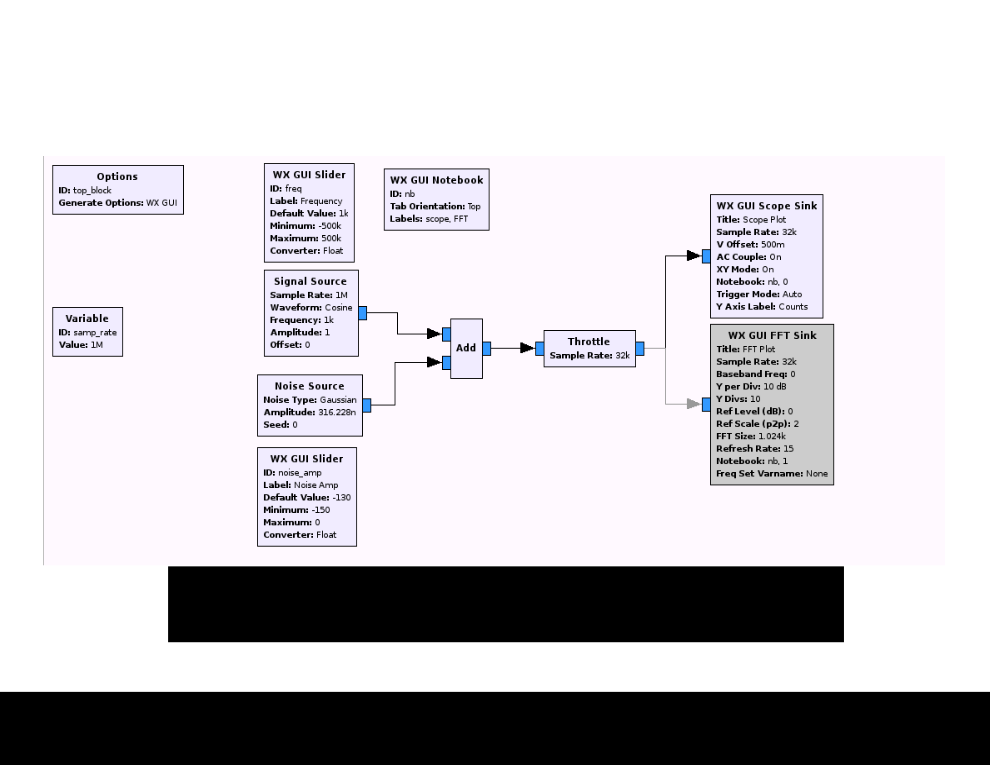
\includegraphics[width=1.2\textwidth]{lab2/pdf/lab2_1.pdf}
\end{figure}
\end{frame}
%---------------------------------

\begin{frame}{Osciloscopio y FFT}
\begin{figure}[H]
\vspace{-4mm}
\centering
\includegraphics[width=1.1\textwidth]{lab2/pdf/lab2_2.pdf}
\end{figure}
\end{frame}
%--------------------------------

\begin{frame}{Osciloscopio y FFT\index{Noise Source}}
\begin{figure}[H]
\centering
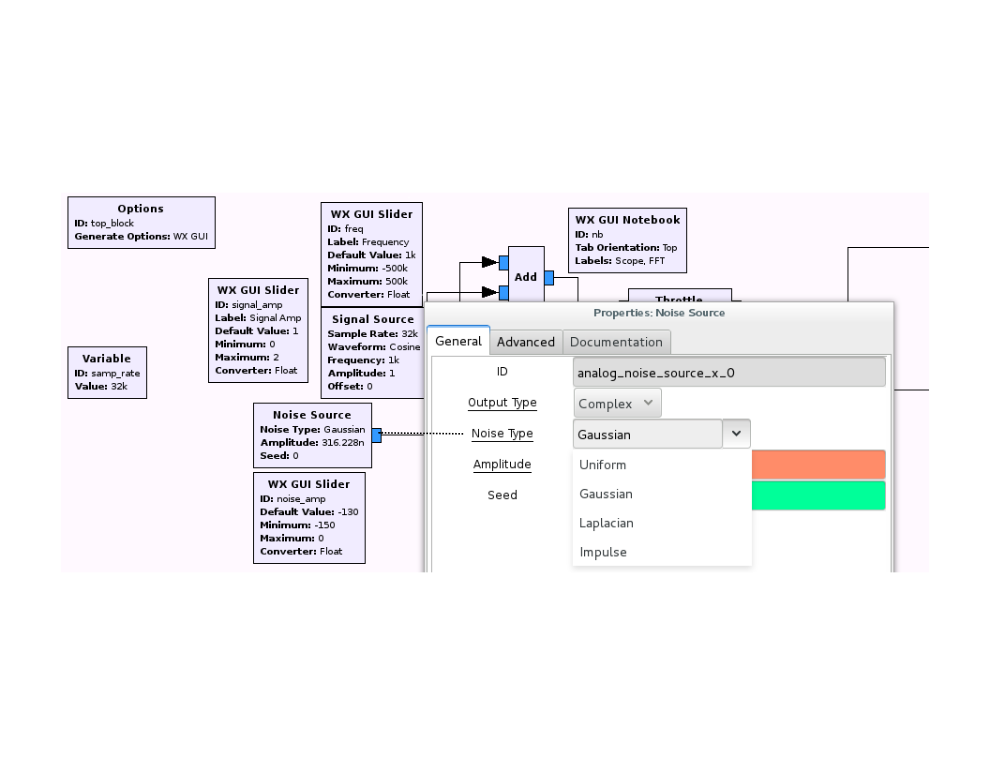
\includegraphics[width=1.055\textwidth]{lab2/pdf/lab2_3.pdf}
\end{figure}
\end{frame}
%--------------------------------

\begin{frame}{Osciloscopio y FFT\index{Noise Source}}
\begin{figure}[H]
\centering
\includegraphics[width=1.055\textwidth]{lab2/pdf/lab2_4.pdf}
\end{figure}
\end{frame}
%--------------------------------

\begin{frame}{Osciloscopio y FFT\index{Add}}
\begin{figure}[H]
\centering
\includegraphics[width=\textwidth]{lab2/pdf/lab2_5.pdf}
\end{figure}
\end{frame}
%--------------------------------

\begin{frame}{Osciloscopio y FFT}
\begin{figure}[H]
\vspace{-4mm}
\centering
\includegraphics[width=1.1\textwidth]{lab2/pdf/lab2_6.pdf}
\end{figure}
\end{frame}
%--------------------------------

\begin{frame}{Osciloscopio y FFT\index{WX GUI Notebook}}
\begin{figure}[H]
\vspace{-4mm}
\centering
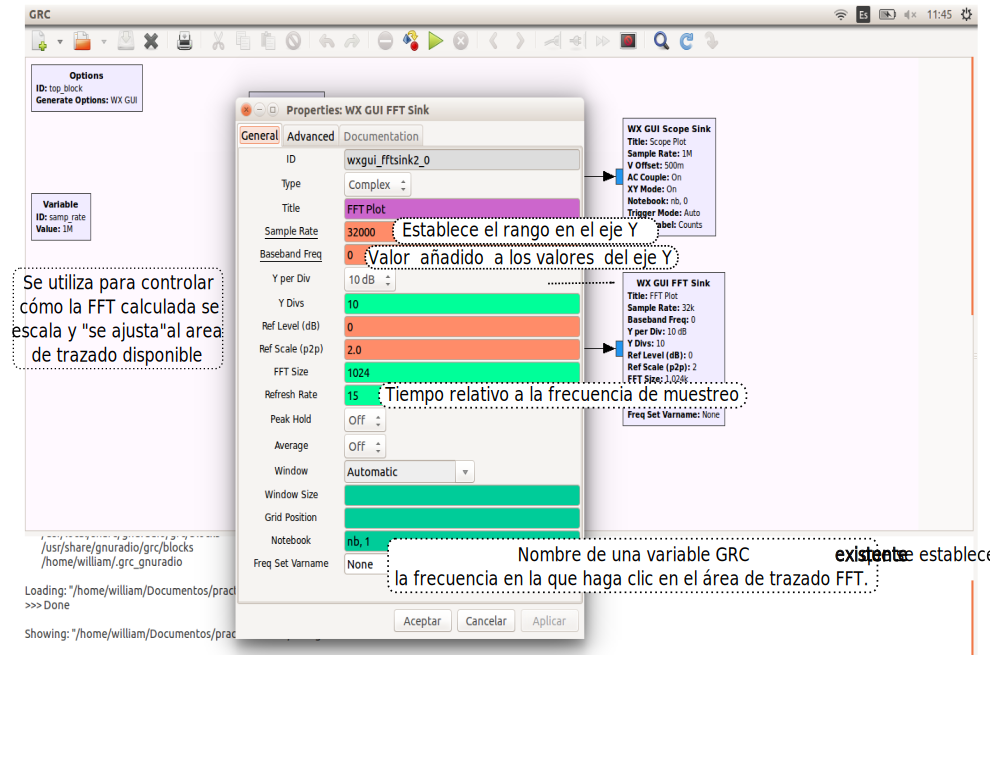
\includegraphics[width=0.85\textwidth]{lab2/pdf/lab2_7.pdf}
\end{figure}
\end{frame}
%--------------------------------

\begin{frame}{Osciloscopio y FFT\index{WX GUI FFT Sink}}
\begin{figure}[H]
\centering
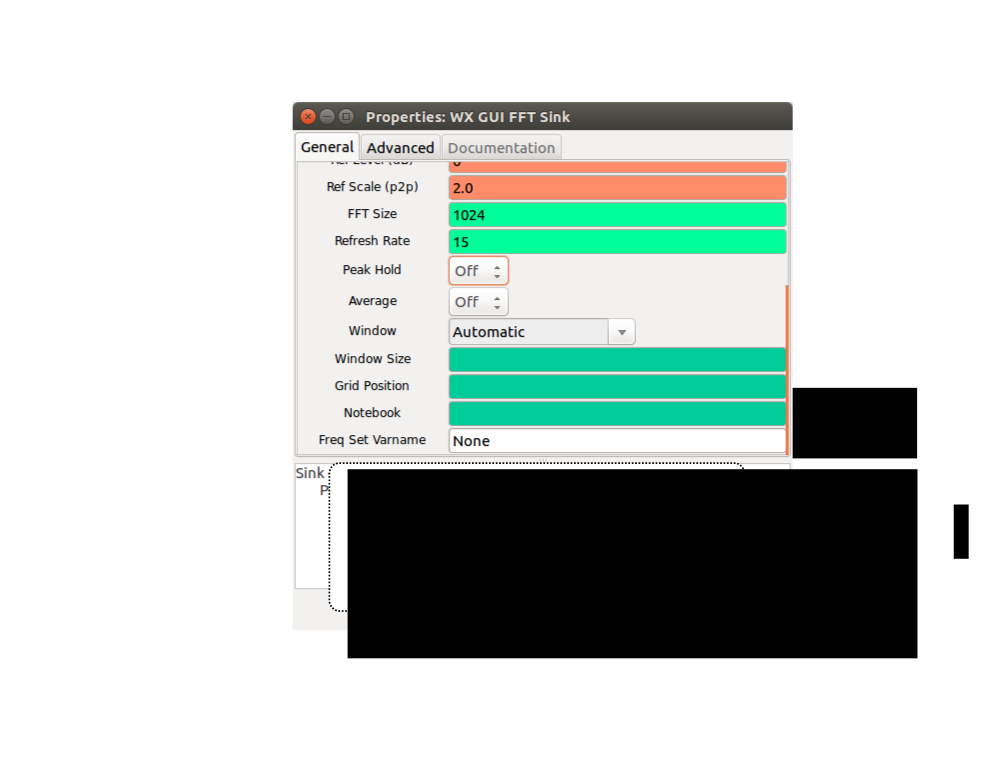
\includegraphics[width=1.1\textwidth]{lab2/pdf/lab2_8.pdf}
\end{figure}
\end{frame}
%--------------------------------

\begin{frame}{Osciloscopio y FFT\index{WX GUI FFT Sink}}
\begin{figure}[H]
\vspace{-3mm}
\centering
\includegraphics[width=0.7\textwidth]{lab2/pdf/lab2_9.pdf}
\end{figure}
\end{frame}
%--------------------------------

\begin{frame}{Osciloscopio y FFT}
\begin{figure}[H]
\vspace{-3mm}
\centering
\includegraphics[width=0.85\textwidth]{lab2/pdf/lab2_10.pdf}
\end{figure}
\end{frame}
%--------------------------------

\begin{frame}{Osciloscopio y FFT}
\begin{figure}[H]
\vspace{-3mm}
\centering
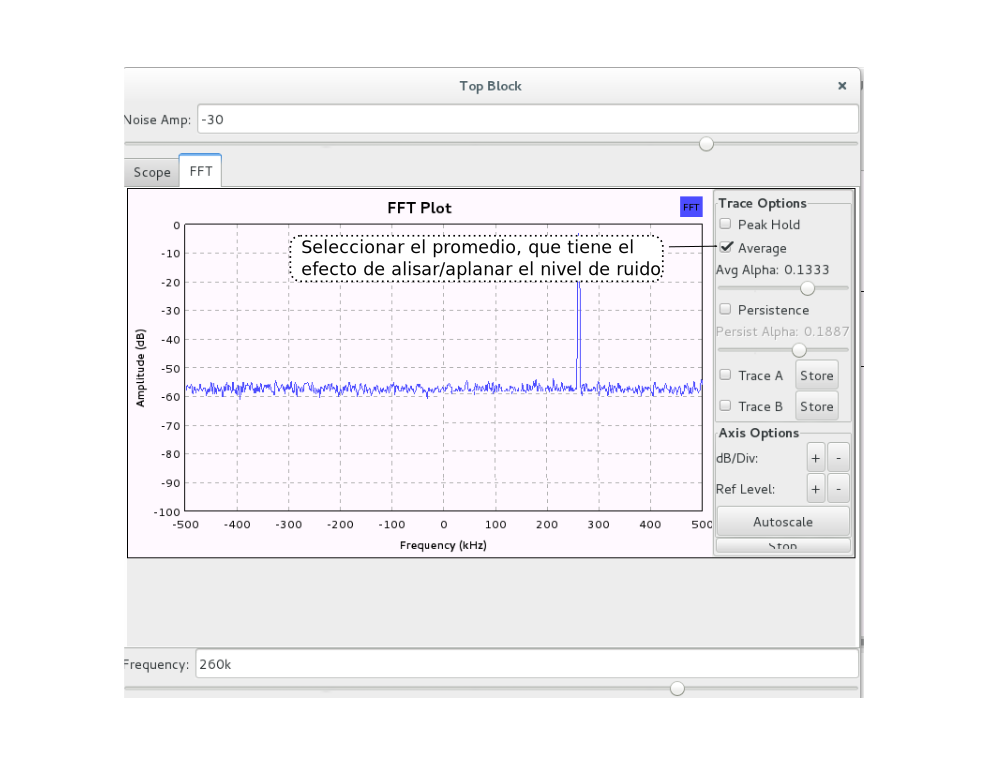
\includegraphics[width=0.75\textwidth]{lab2/pdf/lab2_11.pdf}
\end{figure}
\end{frame}
%--------------------------------

\begin{frame}{Osciloscopio y FFT}
\begin{figure}[H]
\vspace{-3mm}
\centering
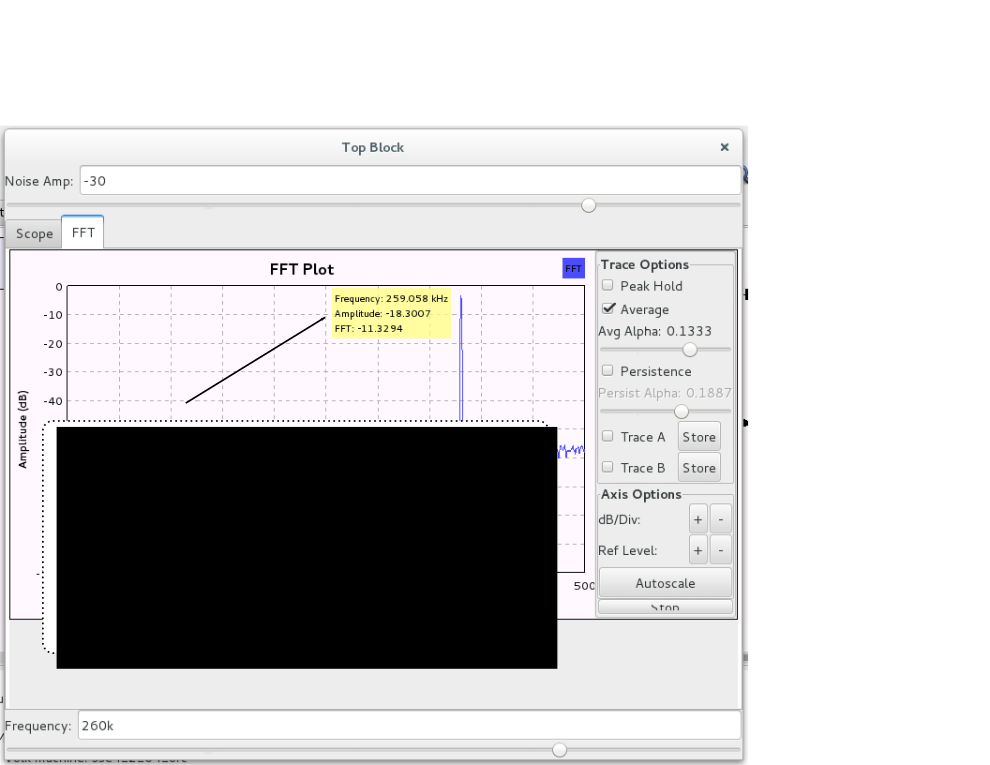
\includegraphics[width=0.75\textwidth]{lab2/pdf/lab2_12.pdf}
\end{figure}
\end{frame}
%--------------------------------

\begin{frame}{Osciloscopio y FFT}
\begin{figure}[H]
\centering
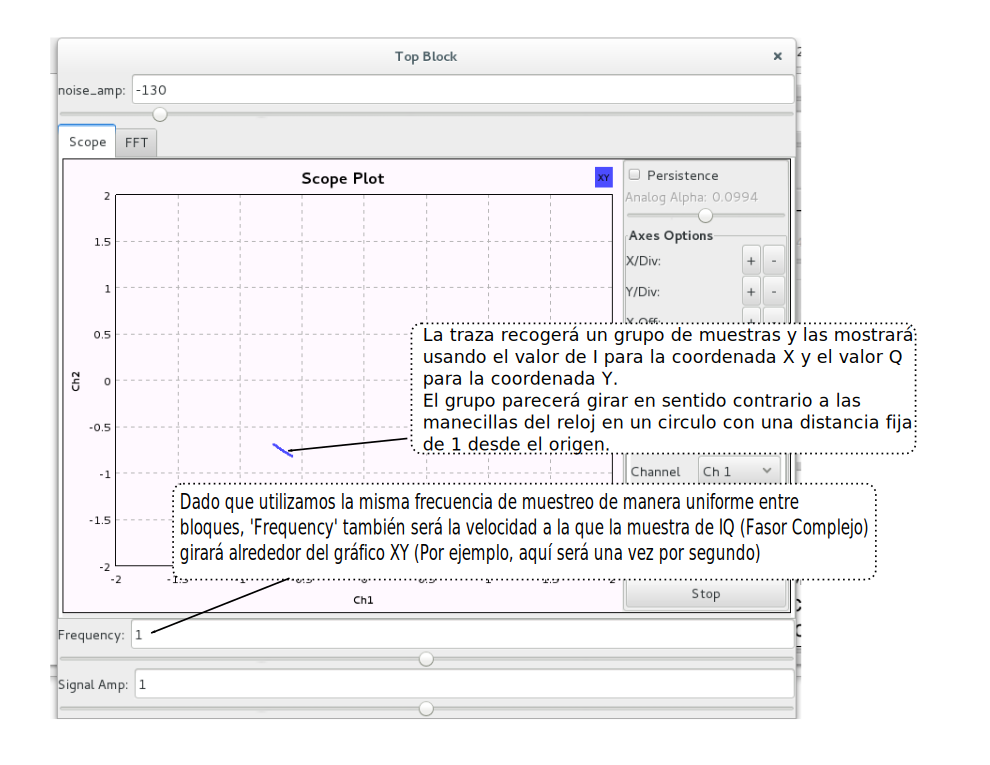
\includegraphics[width=0.75\textwidth]{lab2/pdf/lab2_13.pdf}
\end{figure}
\end{frame}
%--------------------------------

\begin{frame}{Osciloscopio y FFT}
\begin{figure}[H]
\vspace{-3mm}
\centering
\includegraphics[width=0.75\textwidth]{lab2/pdf/lab2_14.pdf}
\end{figure}
\end{frame}
%--------------------------------

\begin{frame}{Osciloscopio y FFT}
\begin{figure}[H]
\vspace{-3mm}
\centering
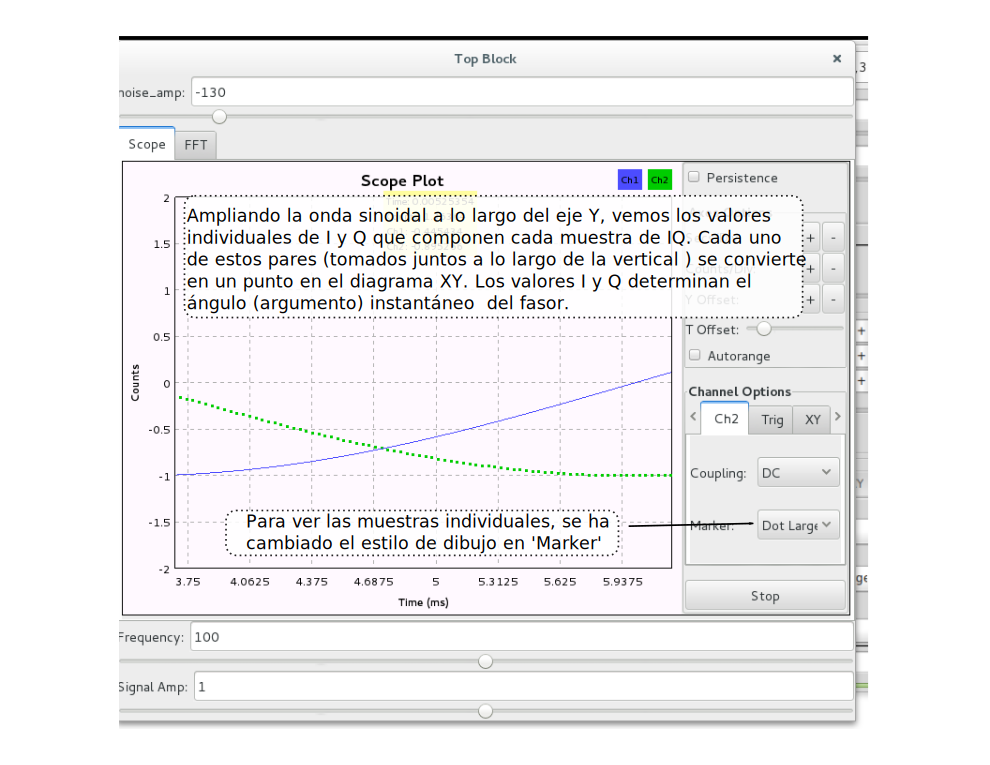
\includegraphics[width=0.7\textwidth]{lab2/pdf/lab2_15.pdf}
\end{figure}
\end{frame}
%--------------------------------

\begin{frame}{Osciloscopio y FFT}
\begin{figure}[H]
\centering
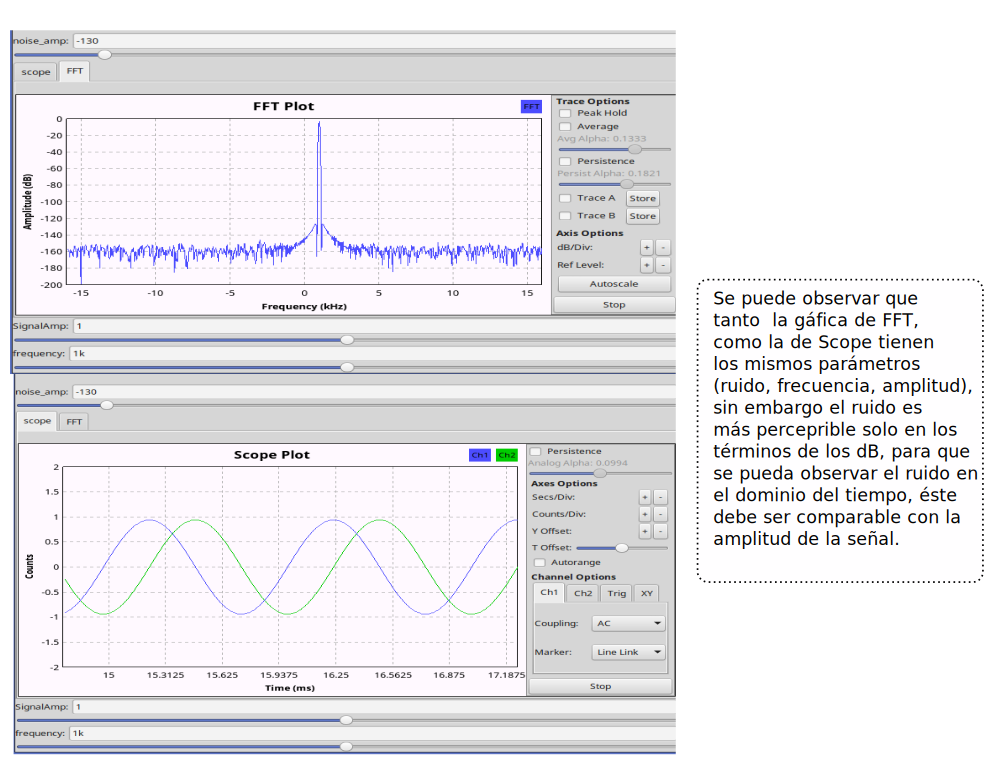
\includegraphics[width=\textwidth, height=0.58\textwidth]{lab2/pdf/lab2_16.pdf}
\end{figure}
\end{frame}
%--------------------------------

%///////////////////////////////////////////////////////////////

\section{Lab3: Audio}
%*********************
\begin{frame}{}

\pgfdeclareimage[width=\paperwidth,height=\paperheight]{bg}{imagenes/fondocap2}
\setbeamertemplate{background}{\pgfuseimage{bg}}

\bfseries{\textrm{\LARGE Lab3\\ \Large Audio}}
\raggedright
\end{frame}
%*********************

\begin{frame}{Audio - Resumen\index{Audio}}

\pgfdeclareimage[width=\paperwidth,height=\paperheight]{bg}{imagenes/fondo3}
\setbeamertemplate{background}{\pgfuseimage{bg}}


En esta práctica se generará un tono desde la tarjeta de sonido de la computadora, originado desde el software y emitido a través de los parlantes del computador, dicha señal sera visualizada desde un osciloscopio, un FFT, y diagrama de cascada (espectrograma), realizando pruebas de "loopback" usando el micrófono de la computadora.

\end{frame}
%----------------

\begin{frame}{Audio\index{Audio}}

Diagrama general: “generación de audio desde la tarjeta de sonido de la computadora”

\begin{figure}

\begin{center}
\vspace{-0.3cm}
\includegraphics[width=.7\textwidth]{lab3/pdf/lab3_1.pdf}
\end{center}
\end{figure}

\end{frame}
%----------------

\begin{frame}{Audio\index{Audio}}

\begin{figure}

\begin{center}
\vspace{-2mm}
    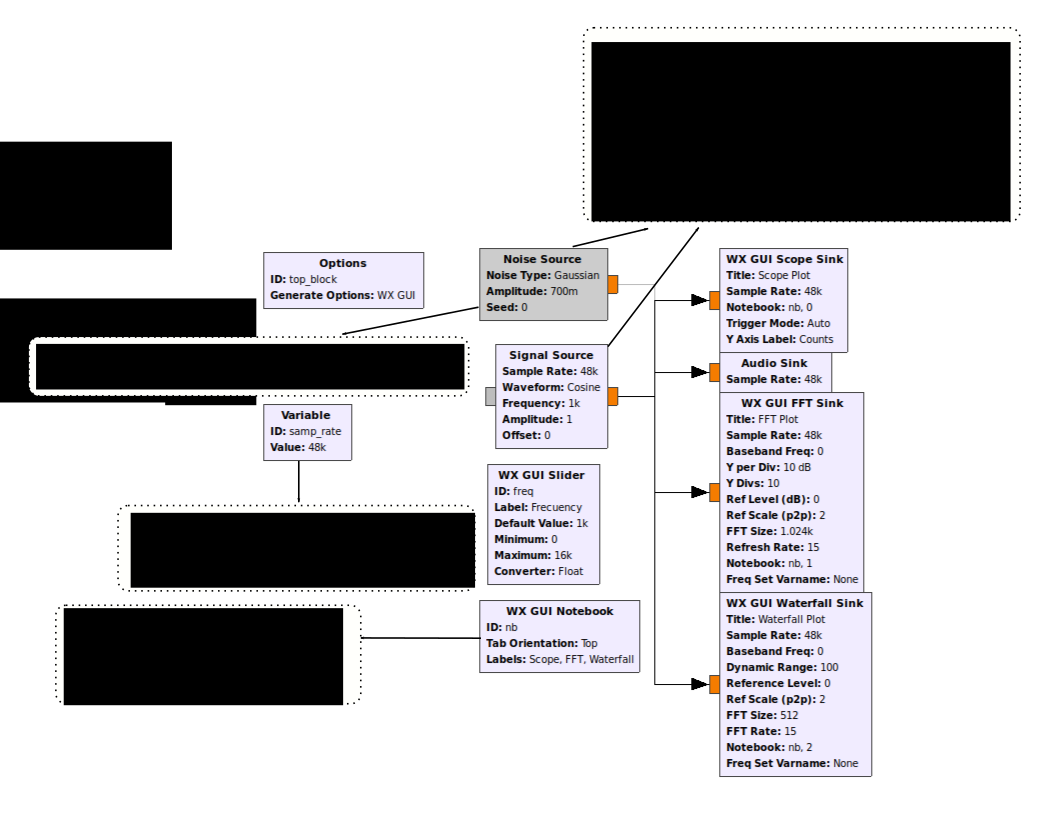
\includegraphics[width=.85\textwidth]{lab3/pdf/lab3_2.pdf}
\end{center}
\end{figure}

\end{frame}
%----------------

\begin{frame}{Audio\index{Audio}}

\begin{figure}

\begin{center}
\vspace{-1mm}
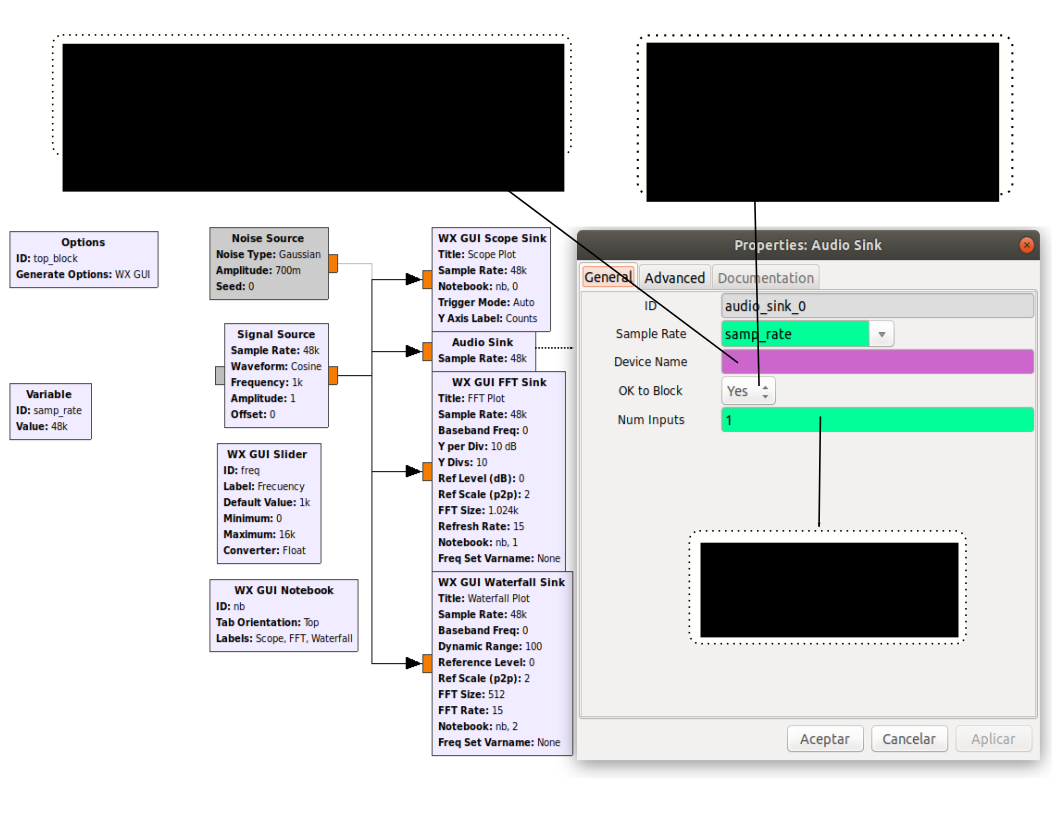
\includegraphics[width=.92\textwidth]{lab3/pdf/lab3_3.pdf}
\end{center}
\end{figure}

\end{frame}
%----------------

\begin{frame}{Audio\index{Audio}}

\begin{figure}

\begin{center}
\vspace{-8mm}
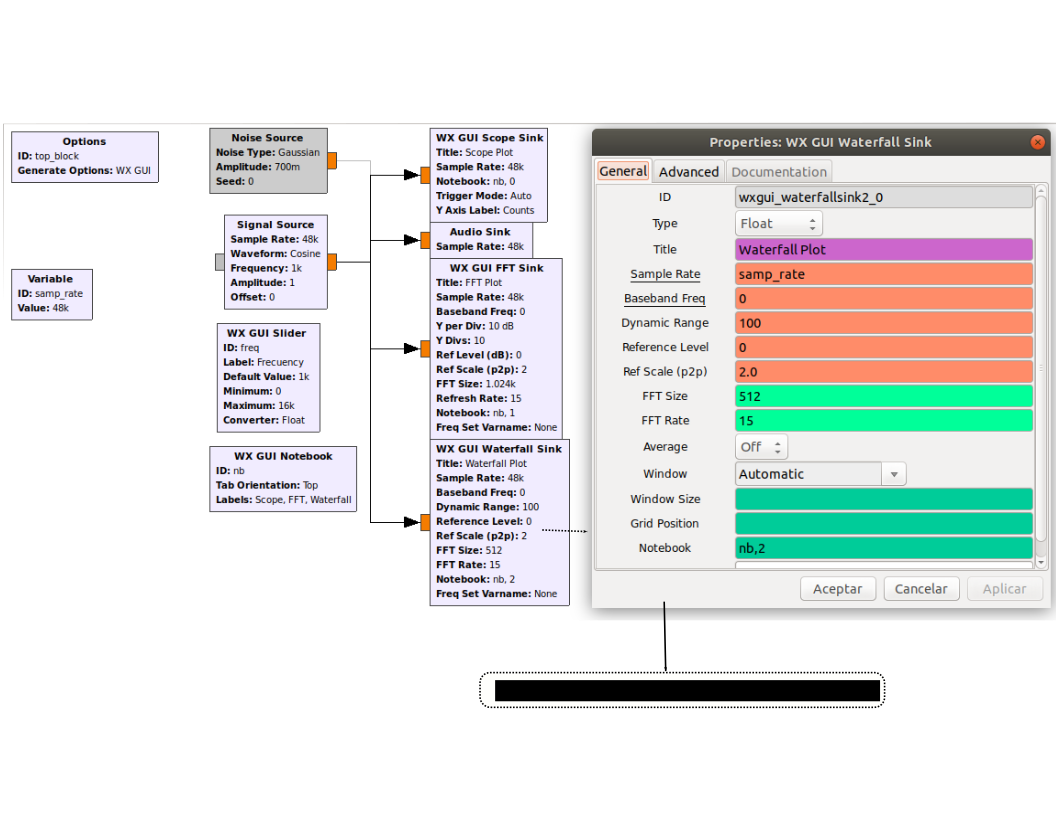
\includegraphics[width=1.05\textwidth]{lab3/pdf/lab3_4.pdf}
\end{center}
\end{figure}

\end{frame}
%----------------

\begin{frame}{Audio - Resumen\index{Audio}}

Es importante saber que:\\
\begin{itemize}
    \item
    {El modo de bloqueo (‘OK to Block’) aplicará previamente un controlador regulado para que el Audio Sink opere eficazmente al escuchar el sonido, además es el único dispositivo del hardware en el diagrama de bloques capaz de emitir audio.}
    \item
    {Esto puede ser problemático si la fuente del diagrama de flujo es, por ejemplo, un RTL-SDR. La fuente es también un hardware que tiene su propio reloj interno y será regulado a la tasa de producción de las muestras, mientras que el Audio Sink regula el uso con su propio reloj no sincronizado. Esto se llama el problema de “dos relojes".}
\end{itemize}
\end{frame}
%----------------

\begin{frame}{Audio - Resumen\index{Audio}}
\begin{itemize}
    \item 
    {Para solucionar este problema de dos relojes, se coloca un regulador de audio en modo sin bloqueo (no dar click ‘Botón de Bloqueo’) de tal forma que nunca interrumpa el diagrama de bloque (es decir, no aplicar el regulador controlado). Esto usará muestras de forma normal, pero si hay un exceso (por ejemplo, el RTL-SDR está produciendo muestras un poco más rápido de lo que el Audio Sink puede usar), se caerán las muestras (podría causar fallas de audio).}
    \item 
    {Esto no soluciona el caso en el que las muestras se producen más lentamente que la tasa de uso del Audio Sink (esto producirá una ejecución lenta: el audio sonará agitado y se imprimirá ‘aU’ en la ventana de registro).}
\end{itemize}



\end{frame}
%----------------

\begin{frame}{Audio\index{Audio}}

\begin{figure}

\begin{center}
\vspace{-7mm}
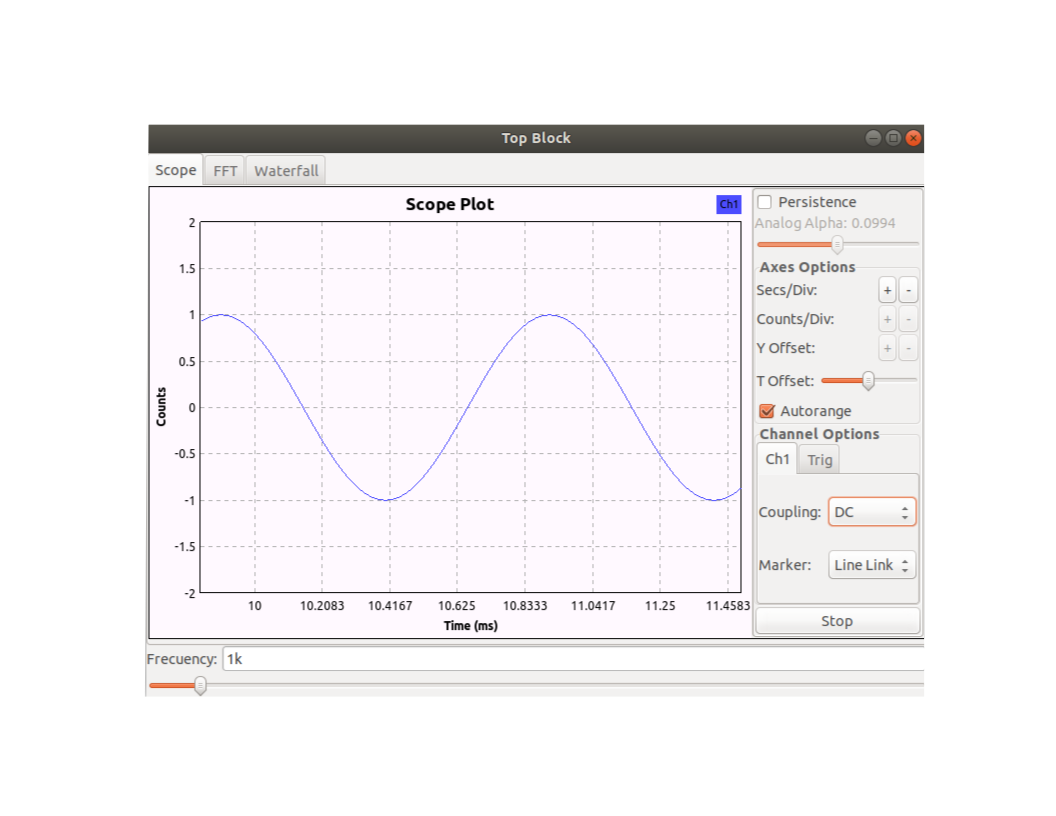
\includegraphics[width=\textwidth, height=0.6\paperheight]{lab3/pdf/lab3_5.pdf}
\end{center}
\end{figure}
%\tiny
\vspace{-4mm}
La misma onda seno de las prácticas anteriores, pero ahora se puede escuchar emitida por los parlantes del computador.
\end{frame}
%----------------

\begin{frame}{Audio\index{Audio}}

\begin{figure}

\begin{center}
\vspace{-6mm}
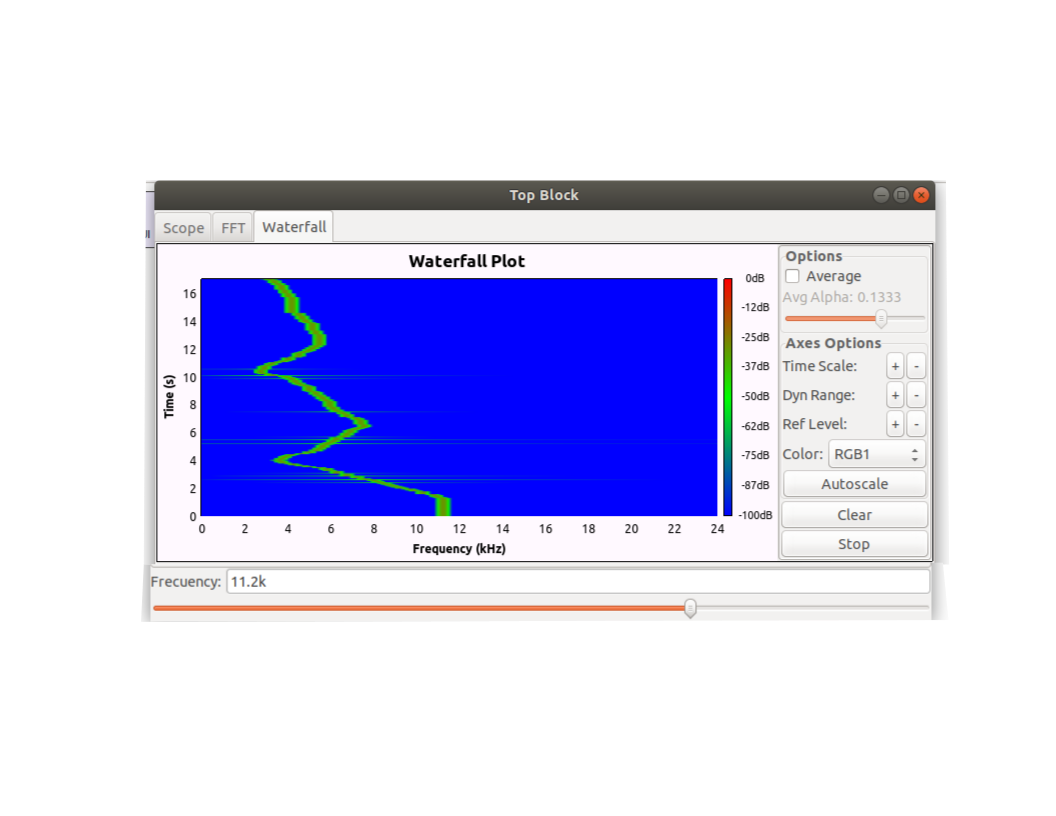
\includegraphics[width=0.8\textwidth]{lab3/pdf/lab3_6.pdf}
\end{center}
\end{figure}
\vspace{-3mm}
\tiny
Visualiza el FFT que se desplaza en el tiempo mediante el diagrama de cascada (espectograma) de la señal emitida. Se añade un bloque de prueba por medio de un generador de señales y un variador deslizante con lo cual se escucha el tono variado en el Audio Sink y poder ver la variación de la frecuencia en el diagrama de cascada.
\end{frame}
%----------------

\begin{frame}{Audio\index{Audio}}
\scriptsize
Recepción de audio - diagrama general
\begin{figure}

\begin{center}
%\vspace{-5mm}
\includegraphics[width=.73\textwidth]{lab3/pdf/lab3_7.pdf}
\end{center}
\end{figure}

\end{frame}
%----------------

\begin{frame}{Audio\index{Audio}}

\begin{figure}
\begin{center}
\vspace{-8mm}
\includegraphics[width=\textwidth, height=0.65\paperheight]{lab3/pdf/lab3_8.pdf}
\end{center}
\end{figure}
\vspace{-2cm}
Muestra las diferentes señales presentes en el entorno captadas por la tarjeta de audio de la computadora a través del micrófono.

\end{frame}
%----------------

\begin{frame}{Audio\index{Audio}}
\scriptsize
Diagrama prueba con aproximación de “loopback”
\begin{figure}
\begin{center}
\vspace{-6mm}
\includegraphics[width=\textwidth, height=0.6\paperheight]{lab3/pdf/lab3_9.pdf}
\end{center}
\end{figure}
\vspace{-5mm}
\tiny
Ejecutando el programa generador de onda sinusoidal al mismo tiempo, y cambiando la frecuencia. Se trata de una prueba aproximada de “loopback" en la que el micrófono de la computadora escucha sus altavoces.

\end{frame}
%----------------

\begin{frame}{Audio\index{Audio}}

\begin{figure}
\begin{center}
\vspace{-8mm}
\includegraphics[width=\textwidth, height=0.6\paperheight]{lab3/pdf/lab3_10.pdf}
\end{center}
\end{figure}
\vspace{-5mm}
\tiny
Con la retro-alimentación de las entradas micrófono-altavoces y generación de señal a través de la tarjeta de audio de la computadora.

\end{frame}
%---------------


%///////////////////////////////////////////////////////////////

\section{Lab4: Modulación ASK en GRC}

%*********************
\begin{frame}{}

\pgfdeclareimage[width=\paperwidth,height=\paperheight]{bg}{imagenes/fondocap2}
\setbeamertemplate{background}{\pgfuseimage{bg}}

\bfseries{\textrm{\LARGE Lab4\\ \Large Modulación ASK en GRC}}
\raggedright
\end{frame}
%*********************


\begin{frame}{Modulación ASK en GRC}

\pgfdeclareimage[width=\paperwidth,height=\paperheight]{bg}{imagenes/fondo3}
\setbeamertemplate{background}{\pgfuseimage{bg}}


\begin{figure}[H]
\centering
\includegraphics[width=\textwidth]{lab4/pdf/lab4_1.pdf}
\end{figure}
\end{frame}
%--------------------

\begin{frame}{Modulación ASK en GRC}
\begin{figure}[H]
\centering
\includegraphics[width=\textwidth]{lab4/pdf/lab4_2.pdf}
\end{figure}
\end{frame}
%_---------------------

\begin{frame}{Modulación ASK en GRC}
\begin{figure}[H]
\centering
\includegraphics[width=\textwidth]{lab4/pdf/lab4_3.pdf}
\end{figure}
\end{frame}
%_---------------------

\begin{frame}{Modulación ASK en GRC}
\begin{figure}[H]
\centering
\includegraphics[width=\textwidth]{lab4/pdf/lab4_4.pdf}
\end{figure}
\end{frame}
%_---------------------

\begin{frame}{Modulación ASK en GRC}
\begin{figure}[H]
\centering
\includegraphics[width=\textwidth]{lab4/pdf/lab4_5.pdf}
\end{figure}
\end{frame}
%_---------------------

\begin{frame}{Modulación ASK en GRC}
\begin{figure}[H]
\centering
\includegraphics[width=\textwidth]{lab4/pdf/lab4_6.pdf}
\end{figure}
\end{frame}
%_---------------------

%///////////////////////////////////////////////////////////////

\section{Lab5: Modulación BPSK en GRC}

%*********************
\begin{frame}{}

\pgfdeclareimage[width=\paperwidth,height=\paperheight]{bg}{imagenes/fondocap2}
\setbeamertemplate{background}{\pgfuseimage{bg}}

\bfseries{\textrm{\LARGE Lab5\\ \Large Modulación BPSK en GRC}}
\raggedright
\end{frame}
%*********************

\begin{frame}{Modulación BPSK en GRC}

\pgfdeclareimage[width=\paperwidth,height=\paperheight]{bg}{imagenes/fondo3}
\setbeamertemplate{background}{\pgfuseimage{bg}}
\begin{figure}
  \centering
   \includegraphics[width=.8\textwidth]{lab5/pdf/lab5_1.pdf}
  \end{figure}
\end{frame}
%------------------------

\begin{frame}{Modulación BPSK en GRC}
\begin{figure}[H]
\centering
\includegraphics[width=.7\textwidth]{lab5/pdf/lab5_2.pdf}
\end{figure}
\end{frame}
%------------------------

\begin{frame}{Modulación BPSK en GRC}
\begin{figure}[H]
\centering
\includegraphics[width=\textwidth]{lab5/pdf/lab5_3.pdf}
\end{figure}
\end{frame}
%------------------------

\begin{frame}{Modulación BPSK en GRC}
\begin{figure}[H]
\centering
\includegraphics[width=.8\textwidth]{lab5/pdf/lab5_4.pdf}
\end{figure}
\end{frame}
%------------------------

\begin{frame}{Modulación BPSK en GRC}
\begin{figure}[H]
\centering
\includegraphics[width=\textwidth]{lab5/pdf/lab5_5.pdf}
\end{figure}
\end{frame}
%------------------------

%///////////////////////////////////////////////////////////////

\section{Bibliografía}

%*********************
\begin{frame}{}

\pgfdeclareimage[width=\paperwidth,height=\paperheight]{bg}{imagenes/fondocap2}
\setbeamertemplate{background}{\pgfuseimage{bg}}

\bfseries{\textrm{\LARGE \\Bibliografía}}
\raggedright
\end{frame}
%*********************



\begin{frame}{Bibliografía}

\pgfdeclareimage[width=\paperwidth,height=\paperheight]{bg}{imagenes/fondo3}
\setbeamertemplate{background}{\pgfuseimage{bg}}

\begin{thebibliography}{X}

\bibitem{Baz} \textsc{Khyati Vachhani Assistant Professor}, 
\textit{Design Analysis of Digital Modulation }, Schemes with GNU Radio.


\bibitem{Baz} \textsc{v3l0c1r4pt0r}, 
\textit{RTL-SDR FM Radio Receiver With GNU Radio Companion }


\bibitem{Baz} \textsc{ Dr. Aaron Scher}, 
\textit{GNU Radio Companion - BPSK Pulse shaping}

\bibitem{Baz} \textsc{ Balint Seeber y
Ettus Research}, 
\textit{GNU Radio Tutorials
Labs 1 – 5}

\end{thebibliography}
\end{frame}


\end{document}
